% !TEX program = lualatex
\documentclass[12pt]{article}
\newcommand{\DocShort}{Flujo uniforme en tuberías circulares}
\usepackage{fontspec}
\setmainfont{TeX Gyre Pagella}
\setsansfont{TeX Gyre Heros}
\usepackage[spanish,es-noshorthands]{babel}
\decimalpoint
\usepackage{geometry}
\geometry{letterpaper, top=2.5cm, bottom=2.5cm, left=2.8cm, right=2.8cm}
\usepackage[expansion=false]{microtype}
\usepackage{parskip}
\setlength{\parskip}{6pt}
\usepackage{amsmath,amssymb}
\usepackage{siunitx}
\usepackage{booktabs}
\usepackage{array}
\usepackage{longtable}
\usepackage{tabularx}
\usepackage{caption}
\usepackage[dvipsnames,table]{xcolor}
\usepackage{enumitem}
\setlist[itemize]{topsep=2pt, itemsep=2pt, parsep=0pt}
\setlist[enumerate]{topsep=2pt, itemsep=2pt, parsep=0pt}
\usepackage{fancyhdr}
\usepackage[hidelinks,pdfencoding=auto]{hyperref}
\usepackage{titlesec}
\usepackage{tcolorbox}
\tcbuselibrary{breakable}
\usepackage{pgfplots}
\pgfplotsset{compat=1.18}
\usepackage{tikz}
\usepackage{makecell}
\usepackage{multicol}
\usepackage{graphicx}
\usepackage{float}
\usepackage{needspace}

\sisetup{
  group-separator={,},
  group-minimum-digits=4,
  output-decimal-marker={.}
}

\definecolor{darkblue}{HTML}{1B3A5C}
\definecolor{medblue}{HTML}{2E6DA4}
\definecolor{lightblue}{HTML}{D6E8F7}
\definecolor{teal}{HTML}{1A7A6E}
\definecolor{lightgrey}{HTML}{F5F5F5}
\definecolor{midgrey}{HTML}{6F6F6F}
\definecolor{warnyellow}{HTML}{FFF3CD}
\definecolor{warnline}{HTML}{B36B00}

\titleformat{\section}
{\large\bfseries\color{darkblue}}
{\thesection}{0.75em}{}[{\color{medblue}\titlerule[0.8pt]}]
\titleformat{\subsection}
{\normalsize\bfseries\color{darkblue}}
{\thesubsection}{0.75em}{}
\titleformat{\subsubsection}
{\normalsize\bfseries\color{medblue}}
{\thesubsubsection}{0.75em}{}

\pagestyle{fancy}
\fancyhf{}
\fancyhead[L]{\small\color{midgrey}ICV 442 Acueductos y Alcantarillados}
\fancyhead[R]{\small\color{midgrey}\DocShort}
\fancyfoot[C]{\small\color{midgrey}\thepage}
\setlength{\headheight}{14pt}
\renewcommand{\headrulewidth}{0.4pt}
\renewcommand{\footrulewidth}{0pt}

\rowcolors{2}{lightgrey}{white}
\renewcommand{\arraystretch}{1.18}

\newtcolorbox{infobox}{
  breakable,
  colback=lightblue,
  colframe=medblue,
  boxrule=0.8pt,
  arc=3pt,
  left=8pt,
  right=8pt,
  top=7pt,
  bottom=7pt
}

\newtcolorbox{warnbox}{
  colback=warnyellow,
  colframe=warnline,
  boxrule=0.8pt,
  arc=3pt,
  left=8pt,
  right=8pt,
  top=7pt,
  bottom=7pt
}

\newcommand{\doccover}[2]{
  \begin{center}
  {\small\color{midgrey}Pontificia Universidad Católica Madre y Maestra\\Escuela de Ingeniería Civil y Ambiental}

  \vspace{1.0cm}
  {\color{medblue}\rule{\linewidth}{2pt}}
  \vspace{0.3cm}

  {\Large\bfseries\color{darkblue}ICV-442-T Acueductos y Alcantarillado}\\[0.35em]
  {\LARGE\bfseries\color{darkblue}#1}

  \vspace{0.3cm}
  {\color{medblue}\rule{\linewidth}{2pt}}
  \vspace{0.9cm}
  \end{center}

  \begin{center}
  \begin{tabular}{ll}
  \toprule
  \textbf{Asignatura} & ICV-442-T Acueductos y Alcantarillado \\
  \textbf{Profesor} & Ricardo Rafael Hernández Moreira, PhD \\
  \textbf{Versión} & #2 \\
  \bottomrule
  \end{tabular}
  \end{center}

  \vspace{0.4cm}
}

\newcommand{\introbox}[2]{
  \begin{infobox}
  \textbf{Propósito.} #1

  \vspace{0.55\baselineskip}

  \textbf{Qué se espera.} #2
  \end{infobox}
}

\newcommand{\deliverablebox}[1]{
  \begin{warnbox}
  \textbf{Entrega.} #1
  \end{warnbox}
}

\AtBeginDocument{
  \hypersetup{
    pdftitle={\DocShort},
    pdfauthor={Ricardo Rafael Hernández Moreira},
    pdfsubject={ICV 442 Acueductos y Alcantarillados}
  }
}


\begin{document}
\doccover{Herramienta de Excel para flujo uniforme en tuberías circulares}{2026-07}
\introbox{Usted construirá una herramienta de Excel que represente la geometría de una tubería circular parcialmente llena, aplique la ecuación de Manning y determine la profundidad normal para un caudal especificado.}{Usted entregará un libro trazable, robusto y fácil de verificar que compare los modelos de rugosidad constante y variable, identifique raíces múltiples y documente sus pruebas dentro del propio archivo.}

\section{Naturaleza de la actividad}
\begin{itemize}
\item Modalidad: individual.
\item Producto central: un libro de Excel con fórmulas visibles, resultados, gráficas y pruebas.
\item Sistema de unidades: Sistema Internacional (SI).
\item Plataforma prevista: Excel 365.
\item Restricción principal: no se permite depender de macros, VBA, Buscar objetivo, Solver ni complementos externos.
\end{itemize}

\deliverablebox{El único archivo requerido será un libro con extensión \texttt{.xlsx}. Toda explicación necesaria para comprender el método, los supuestos, las advertencias y las pruebas deberá estar incorporada dentro del propio libro.}

\section{Resultados de aprendizaje}
Al completar la asignación, usted deberá ser capaz de:
\begin{itemize}
\item traducir relaciones geométricas e hidráulicas a fórmulas de Excel correctamente referenciadas;
\item calcular parámetros de flujo uniforme para un tirante conocido;
\item resolver numéricamente la profundidad normal mediante fórmulas auditables;
\item reconocer cuándo un caudal admite una, dos o ninguna profundidad a superficie libre;
\item verificar resultados mediante casos límite, valores de control y pruebas de ida y vuelta.
\end{itemize}

\section{Fundamento geométrico}
Considere una tubería circular de diámetro $D$, con tirante $y$ medido desde el fondo. Defina la profundidad relativa
\[
x=\frac{y}{D}, \qquad 0\leq x\leq 1,
\]
y trabaje con el ángulo central $\theta$ expresado en radianes.

Para la sección circular parcialmente llena, use las siguientes relaciones:
\begin{align}
\theta &= 2\cos^{-1}\!\left(1-\frac{2y}{D}\right), \\
A &= \frac{D^2}{8}\left(\theta-\sin\theta\right), \\
P &= \frac{D\theta}{2}, \\
R &= \frac{A}{P}, \\
B &= D\sin\left(\frac{\theta}{2}\right)=2\sqrt{y(D-y)}, \\
D_h &= \frac{A}{B}.
\end{align}

En estas expresiones, $A$ es el área de flujo, $P$ el perímetro mojado, $R$ el radio hidráulico, $B$ el ancho de la superficie libre y $D_h$ la profundidad hidráulica.

\begin{figure}[H]
\centering
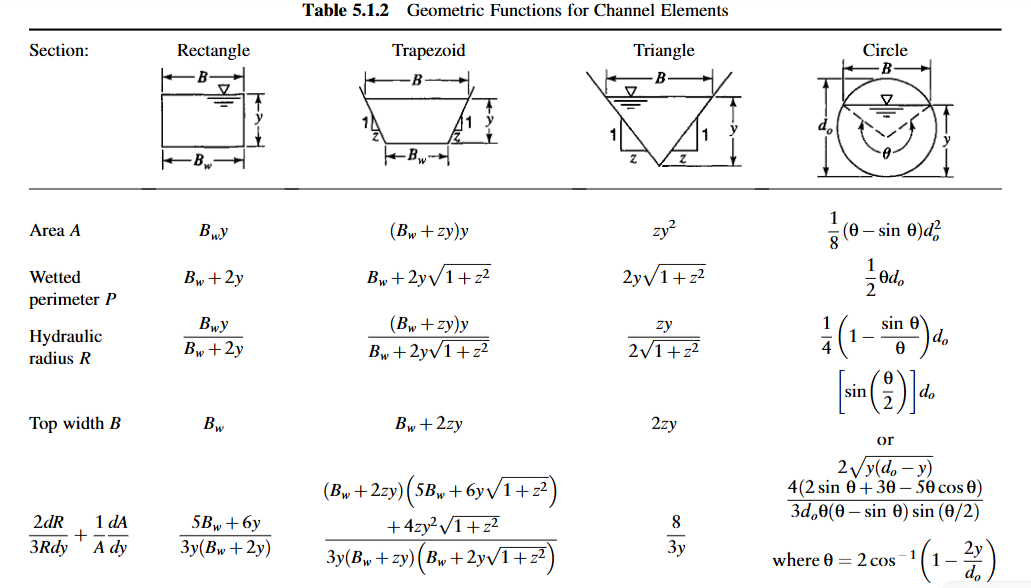
\includegraphics[width=0.86\textwidth]{figura_propiedades_geometricas.png}
\caption{Funciones geométricas para elementos de canal. En esta asignación se utilizará la columna correspondiente a la sección circular.}
\label{fig:geometria}
\end{figure}

\section{Flujo uniforme y propiedades hidráulicas}
La velocidad media y el caudal se calcularán mediante la ecuación de Manning en unidades SI:
\begin{align}
V &= \frac{1}{n}R^{2/3}S_0^{1/2}, \\
Q &= AV,
\end{align}
donde $S_0$ es la pendiente de fondo y $n$ el coeficiente de rugosidad de Manning.

Su herramienta también deberá calcular la energía específica y el número de Froude:
\begin{align}
E &= y+\frac{V^2}{2g}, \\
Fr &= \frac{V}{\sqrt{gD_h}}.
\end{align}

El régimen se clasificará como subcrítico si $Fr<1$, crítico si $Fr\approx 1$ y supercrítico si $Fr>1$. La tolerancia adoptada para identificar el caso crítico deberá aparecer explícitamente en el libro.

\section{Modelos de rugosidad}
Su herramienta deberá resolver y comparar simultáneamente dos modelos.

\subsection{Coeficiente de Manning constante}
Se supondrá
\[
n=n_f,
\]
donde el subíndice $f$ identifica la condición de sección llena.

\subsection{Coeficiente de Manning variable}
Se utilizará la aproximación
\begin{equation}
\frac{n}{n_f}=1+\left(\frac{y}{D}\right)^{0.54}
-\left(\frac{y}{D}\right)^{1.2}.
\end{equation}

\subsection{Relaciones normalizadas}
Como la velocidad de Manning es inversamente proporcional a $n$, use las siguientes relaciones parciales:
\begin{align*}
\frac{V}{V_f} &= \frac{n_f}{n}\left(\frac{R}{R_f}\right)^{2/3}, \\
\frac{Q}{Q_f} &= \frac{n_f}{n}\frac{A}{A_f}
\left(\frac{R}{R_f}\right)^{2/3}.
\end{align*}

\section{Libro de Excel requerido}
Su libro deberá contener, como mínimo, las hojas indicadas en la Tabla~\ref{tab:hojas}. Puede añadir hojas auxiliares, pero no deberá ocultar cálculos esenciales.

\begin{table}[H]
\centering
\caption{Estructura mínima del libro de Excel.}
\label{tab:hojas}
\begin{tabularx}{\textwidth}{>{\raggedright\arraybackslash}p{0.23\textwidth} >{\raggedright\arraybackslash}X}
\toprule
\textbf{Hoja} & \textbf{Contenido requerido} \\
\midrule
Calculadora & Entradas de $D$, $S_0$, $n_f$, $g$, tirante conocido y caudal objetivo; resultados comparativos para ambos modelos. \\
Geometría y flujo & Tabla trazable de $y/D$, $\theta$, $A$, $P$, $R$, $B$, $D_h$, $n/n_f$, $V$, $Q$, $E$, $Fr$, $V/V_f$ y $Q/Q_f$. \\
Profundidad normal & Proceso numérico, residuales, límites de búsqueda y una o dos soluciones según corresponda. \\
Gráficas & Curvas comparativas de $Q/Q_f$, $V/V_f$ y $n/n_f$ contra $y/D$, con ejes, leyenda y escalas correctas. \\
Validación & Casos de prueba, valores esperados, valores calculados, error, tolerancia y estado \emph{Cumple/No cumple}. \\
\bottomrule
\end{tabularx}
\end{table}

\subsection{Requisitos de la interfaz}
\begin{itemize}
\item Diferencie visualmente las entradas, las fórmulas y los resultados.
\item Incluya símbolo, descripción y unidad para todas las entradas y salidas.
\item Valide $D>0$, $S_0>0$, $n_f>0$, $g>0$, $0\leq y\leq D$ y $Q_{\mathrm{obj}}\geq0$.
\item Muestre mensajes comprensibles ante entradas inválidas o casos sin solución.
\item Evite errores visibles como \texttt{\#DIV/0!}, \texttt{\#NUM!}, \texttt{\#VALUE!}, \texttt{\#N/A} o referencias circulares.
\item Mantenga visibles las fórmulas y relaciones de cálculo. No escriba manualmente los resultados clave.
\end{itemize}

\section{Procedimiento mínimo}
\begin{enumerate}
\item Defina las entradas y constantes del problema en celdas independientes y debidamente rotuladas.
\item Construya una discretización de $0\leq y/D\leq1$ con resolución suficiente para cumplir las tolerancias.
\item Calcule la geometría para cada profundidad y trate explícitamente los extremos $y=0$ y $y=D$.
\item Calcule $V$, $Q$, $E$ y $Fr$ para Manning constante y variable, además de las relaciones normalizadas.
\item Determine $Q_f$ y localice $Q_{\max}$ y la profundidad correspondiente para cada modelo.
\item Implemente una búsqueda tabular con interpolación o una bisección de iteraciones fijas para resolver $Q(y)=Q_{\mathrm{obj}}$.
\item Construya las gráficas, ejecute las pruebas de validación y deje evidencia visible del error obtenido.
\end{enumerate}

\section{Profundidad normal y raíces múltiples}
La función $Q(y)$ aumenta hasta un máximo y luego disminuye antes de alcanzar la condición de sección llena. Por tanto, el algoritmo no deberá suponer que $Q(y)$ es monótona en todo el intervalo.

\begin{table}[H]
\centering
\caption{Respuesta requerida según el caudal objetivo.}
\begin{tabularx}{\textwidth}{>{\raggedright\arraybackslash}p{0.22\textwidth} >{\raggedright\arraybackslash}p{0.27\textwidth} >{\raggedright\arraybackslash}X}
\toprule
\textbf{Intervalo} & \textbf{Comportamiento} & \textbf{Respuesta exigida} \\
\midrule
$0\leq Q<Q_f$ & Una solución parcial. & Mostrar la raíz inferior. \\
$Q=Q_f$ & Una raíz parcial y la sección llena. & Mostrar ambas cuando sean distintas dentro de la tolerancia. \\
$Q_f<Q<Q_{\max}$ & Dos soluciones parciales. & Mostrar la raíz inferior y la raíz superior. \\
$Q\approx Q_{\max}$ & Una solución doble. & Unificar las soluciones si difieren menos de $0.001D$. \\
$Q>Q_{\max}$ & Sin solución a superficie libre. & Mostrar una advertencia; no extrapolar. \\
\bottomrule
\end{tabularx}
\end{table}

\begin{infobox}
\textbf{Métodos permitidos.} Su solución deberá actualizarse automáticamente mediante fórmulas. Puede usar una búsqueda tabular con interpolación o una bisección con un número fijo y visible de iteraciones. No deberá depender de Buscar objetivo, Solver, macros VBA ni complementos.

\textbf{Función recomendada.} Le recomendamos explícitamente usar \texttt{XLOOKUP} (\texttt{BUSCARX} en la interfaz de Excel en español) para localizar los valores que encierran el caudal objetivo. Realice la búsqueda por separado en la rama inferior y en la rama superior de $Q(y)$, ya que la relación no es monótona en todo el intervalo.
\end{infobox}

\section{Tratamiento de las fronteras}
\begin{table}[H]
\centering
\caption{Tratamiento de condiciones límite.}
\begin{tabularx}{\textwidth}{>{\raggedright\arraybackslash}p{0.13\textwidth} >{\raggedright\arraybackslash}p{0.38\textwidth} >{\raggedright\arraybackslash}X}
\toprule
\textbf{Condición} & \textbf{Interpretación} & \textbf{Presentación en Excel} \\
\midrule
$y=0$ & $A=0$ y no existe una sección mojada útil. & Mostrar caudal nulo y \texttt{N/A} donde una división no esté definida. \\
$0<y<D$ & Existe una superficie libre definida. & Calcular todas las propiedades, la energía y $Fr$. \\
$y=D$ & $B=0$ y $D_h=A/B$ no está definido como magnitud de superficie libre. & Mostrar \texttt{N/A} para $D_h$ y $Fr$; conservar $A_f$, $P_f$, $R_f$, $V_f$ y $Q_f$. \\
\bottomrule
\end{tabularx}
\end{table}

\section{Gráficas obligatorias}
Se requieren las siguientes gráficas de dispersión XY:
\begin{itemize}
\item $Q/Q_f$ contra $y/D$, con Manning constante y variable en un mismo gráfico;
\item $V/V_f$ contra $y/D$, con Manning constante y variable en un mismo gráfico;
\item $n/n_f$ contra $y/D$ para el modelo variable.
\end{itemize}

Cada gráfica deberá incluir título, rótulos de ejes, leyenda y una escala capaz de mostrar los máximos sin recortar las curvas. Los datos fuente deberán permanecer visibles en el libro.

\section{Validación obligatoria}
La hoja \emph{Validación} deberá calcular el error y determinar automáticamente si cada prueba cumple la tolerancia. Los valores de la Tabla~\ref{tab:validacion} son referencias de control y no sustituyen el desarrollo de las fórmulas.

\begin{longtable}{>{\raggedright\arraybackslash}p{0.25\textwidth} >{\raggedright\arraybackslash}p{0.22\textwidth} >{\raggedright\arraybackslash}p{0.43\textwidth}}
\caption{Casos mínimos de validación.}\label{tab:validacion}\\
\toprule
\textbf{Prueba} & \textbf{Condición} & \textbf{Referencia} \\
\midrule
\endfirsthead
\toprule
\textbf{Prueba} & \textbf{Condición} & \textbf{Referencia} \\
\midrule
\endhead
Media sección & $y/D=0.5$ & $\theta=\pi$; $A/D^2=\pi/8$; $P/D=\pi/2$; $R/D=0.25$. \\
Sección llena & $y/D=1$ & $A_f=\pi D^2/4$; $P_f=\pi D$; $R_f=D/4$; $n/n_f=1$. \\
Velocidad máxima, $n$ constante & Búsqueda del máximo & $y/D\approx0.8128$. \\
Caudal máximo, $n$ constante & Búsqueda del máximo & $y/D\approx0.9382$. \\
Velocidad máxima, $n$ variable & Búsqueda del máximo & $y/D\approx0.9353$. \\
Caudal máximo, $n$ variable & Búsqueda del máximo & $y/D\approx0.9688$. \\
Ida y vuelta & Seleccione un $y/D$ interior. & El $Q$ directo deberá recuperar el mismo $y$ dentro de $0.001D$. \\
\bottomrule
\end{longtable}

\subsection{Tolerancias}
\begin{itemize}
\item Propiedades geométricas, velocidad y caudal: error relativo máximo de \SI{0.5}{\percent}.
\item Profundidad normal: error absoluto máximo de $0.001D$.
\item Máximos: la discretización o búsqueda deberá alcanzar la precisión indicada por los valores de control.
\end{itemize}

\section{Entregable}
\subsection{Archivo requerido}
Entregue un único libro de Excel con extensión \texttt{.xlsx}. Use el nombre:
\begin{center}
\texttt{Apellido\_Nombre\_FlujoUniformeCircular.xlsx}
\end{center}

No se aceptarán libros con vínculos externos rotos, hojas esenciales ocultas o protección que impida revisar las fórmulas. El archivo deberá abrir sin advertencias y recalcular correctamente cuando se modifiquen las entradas.

\Needspace{14\baselineskip}
\section{Rúbrica de evaluación}
{\small
\renewcommand{\arraystretch}{1.05}
\begin{center}
\begin{tabularx}{\textwidth}{>{\raggedright\arraybackslash}p{0.24\textwidth} >{\raggedright\arraybackslash}X >{\raggedleft\arraybackslash}p{0.10\textwidth}}
\toprule
\textbf{Criterio} & \textbf{Evidencia esperada} & \textbf{Puntos} \\
\midrule
Exactitud hidráulica & Geometría, Manning, energía, Froude, unidades y relaciones normalizadas correctas. & 30 \\
Profundidad normal & Automatización, precisión, residuales y manejo correcto de una, dos o ninguna raíz. & 25 \\
Modelos de rugosidad & Implementación y comparación consistente de $n$ constante y variable. & 15 \\
Validación y robustez & Casos de prueba, tolerancias, controles de entrada y ausencia de errores de fórmula. & 15 \\
Organización y presentación & Trazabilidad, rotulación, legibilidad, gráficas y facilidad de uso. & 15 \\
\bottomrule
\end{tabularx}
\end{center}
}

\begin{warnbox}
\textbf{Observaciones de evaluación.}
\begin{itemize}
\item Se calificará tanto el resultado como la trazabilidad del procedimiento.
\item Una cifra correcta sin una fórmula verificable no constituye evidencia suficiente.
\item Su herramienta deberá producir resultados consistentes al cambiar las entradas.
\item Los mensajes de error y advertencia forman parte del funcionamiento esperado.
\end{itemize}
\end{warnbox}

\clearpage
\section{Checklist de revisión rápida}
\begin{longtable}{p{0.95\textwidth}}
\toprule
\textbf{Estructura e interfaz} \\
\midrule
$\square$ Las cinco hojas mínimas están presentes y claramente nombradas. \\
$\square$ Todas las entradas incluyen símbolo, descripción y unidad. \\
$\square$ Las entradas, fórmulas y resultados se distinguen visualmente. \\
\midrule
\textbf{Cálculo hidráulico} \\
\midrule
$\square$ Los dos modelos de rugosidad se actualizan con las mismas entradas. \\
$\square$ La profundidad normal se obtiene sin herramientas manuales ni macros. \\
$\square$ Los casos de dos raíces se detectan y muestran correctamente. \\
$\square$ Los extremos $y=0$ y $y=D$ no producen errores de Excel. \\
\midrule
\textbf{Gráficas y validación} \\
\midrule
$\square$ Las gráficas son XY y muestran los máximos sin recortar las curvas. \\
$\square$ La hoja \emph{Validación} indica automáticamente \emph{Cumple/No cumple}. \\
$\square$ No existen errores de fórmula ni referencias circulares. \\
\midrule
\textbf{Entrega} \\
\midrule
$\square$ El archivo abre, recalcula y conserva sus fórmulas sin vínculos externos. \\
$\square$ El nombre del archivo sigue el formato requerido. \\
\bottomrule
\end{longtable}

\end{document}
